\section{Theory}
\subsection{Short introduction to nuclear and particle physics}
In order to understand the notions of half life period and nuclear fission we
give a short introduction into nuclear and particle physics following \cite{bettini2008introduction}.
In the following, let $Z$ be the atomic number, $N$ the number of neutrons and $A$ the number of nuclei, also
called nucleon number. Thus, $A = Z + N$. The electric charge of the nucleus in the ground state is $+Z e$.
It is common to describe the so called \emph{nuclides} with $_{Z}^{A}\textrm{Y}$.\\
The forces binding the nuclei contribute to the total mass of an atom in terms of the 
binding energy $\Delta E = \Delta M c^2$:
\begin{equation}
\Delta M = M_{tot.} - Z(M_p + M_e) - N M_n \, .
\end{equation}
We used the proton, electron and neutron masses $M_p$, $M_e$ and $M_n$ 
(see figure~\ref{fig:bindingenergy}).
\begin{figure}[htpb]
    \centering
    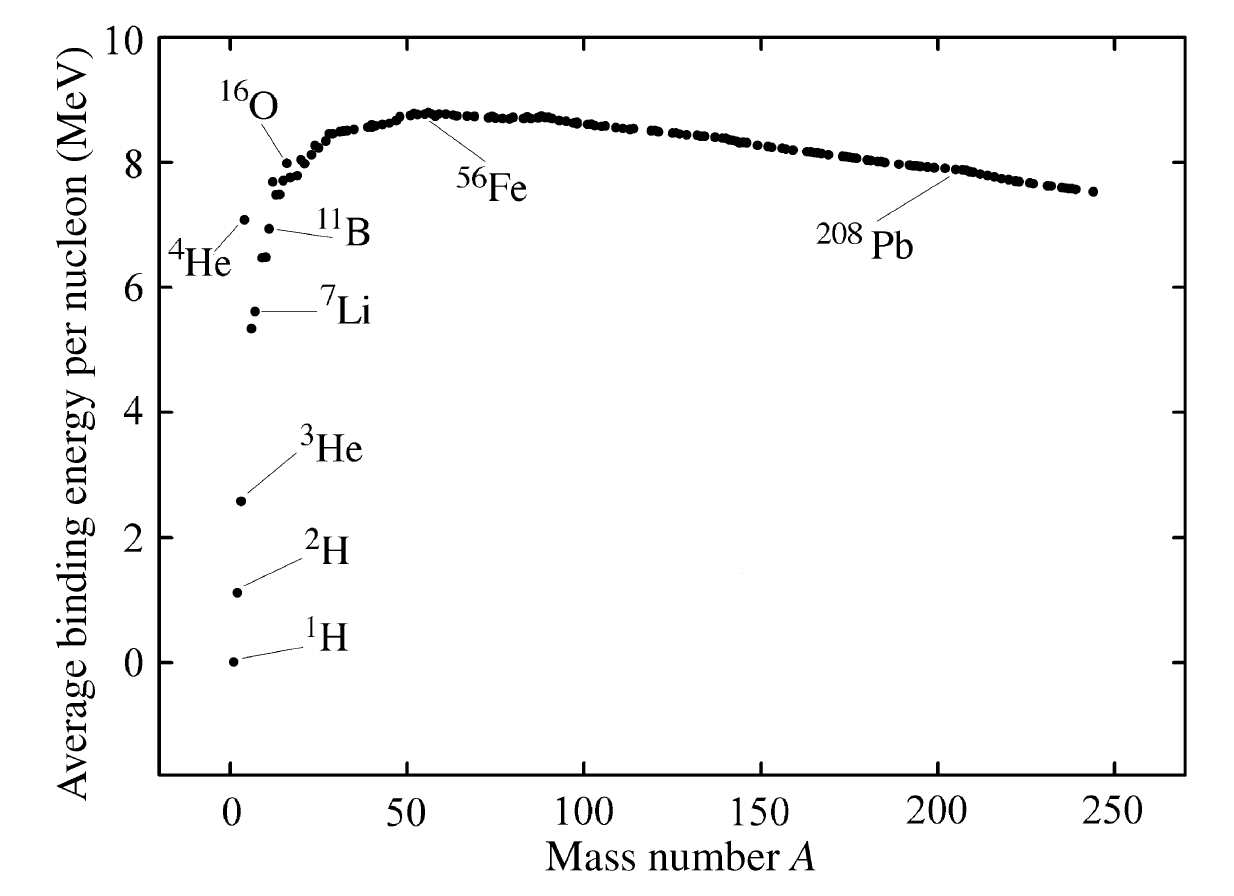
\includegraphics[width=0.8\linewidth]{figures/bindingenergy}
    \caption{Binding energies for nuclei that are stable or long-lived \cite{Hooshyar}.}
    \label{fig:bindingenergy}
\end{figure}
If we look at the distribution of stable nuclei (see figure~\ref{fig:nuclidmap}) we notice
that they occur only in a very narrow band. All other nuclei are unstable and decay spontaneously.
The decay is characerized by a \emph{decay constant} $\lambda$, which is related to the activity $\mathcal{A}$
by 
\begin{equation}\label{eq:decay}
    \mathcal{A} = -\frac{\partial N}{\partial t} = \lambda N 
\end{equation}
where the activity $\mathcal{A}$ is typically given in Bequerel: $1 \textrm{Bq}= \textrm{decay}\cdot s^{-1}$.
A solution to the differential equation \eqref{eq:decay} is
\begin{equation}
    \mathcal{A}(t) = \lambda N_0 \exp(-\lambda t) \, ,
\end{equation}
with the initial condition $N_0 := N(t=t_0)$. 
The probability of an atom to decay within time $t$ is thus
\begin{equation}
    \mathcal{P}(t) = \int_{0}^{t}\lambda \exp(-\lambda t')\mathrm{d}t' = 1 -  \exp(-\lambda t)  \quad
    \textrm{with} \quad \int_{0}^{\infty}\lambda \exp(-\lambda t')\mathrm{d}t' = 1 \, .
\end{equation}
The probability density is accordingly $f(t) = \lambda \exp(-\lambda t)$. 
Hence, we can calculate the expectation value of a random variable $t$ within the probability space
$\Omega$ with the measure  $\mathcal{P}$:
\begin{equation}
    \tau := E[t] = \int_{0}^{\infty} t \lambda \exp(-\lambda t) \mathrm{d}t 
    =\lim_{t \rightarrow \infty}\left[ \frac{exp(-\lambda t) (1-\lambda t) - 1 }{\lambda} \right] 
= \frac{1}{\lambda}
\end{equation}
The half-life $t_{1/2}$ is obviously connected by $t_{1/2}= -\mathrm{log}(2)/ \lambda = - \tau \mathrm{log}(2)$.
\begin{figure}[htpb]
    \centering
    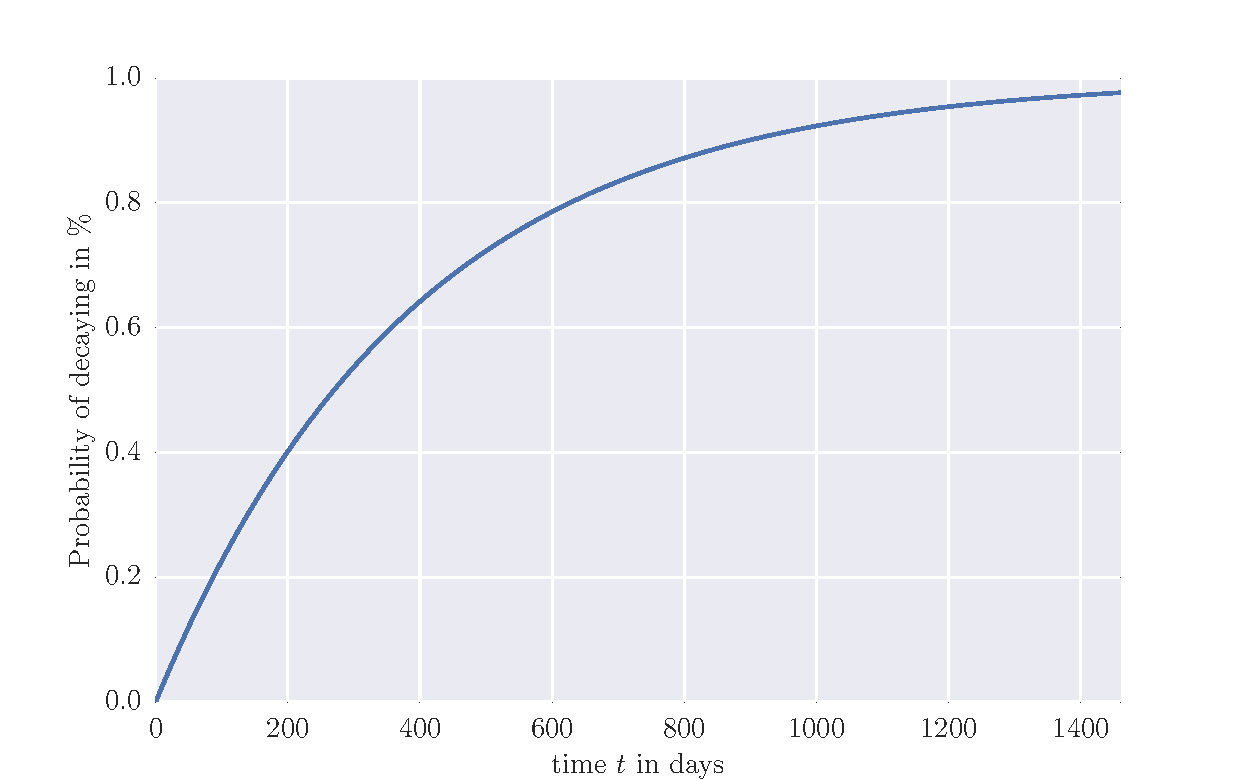
\includegraphics[width=0.9\linewidth]{analysis/figures/halflife}
    \caption{Probability $\mathcal{P}(t) = 1 -  \exp(-\lambda t)$ of an atom to decay within time $t$.
        Here we chose as the decay of
        $^{57}\textrm{Cs}\rightarrow ^{57}\textrm{Fe}$ with $t_{1/2}=270$ over a range
    of 4 years as an example.}
    \label{fig:decay}
\end{figure}
\clearpage
\subsubsection{Semi-Empirical Mass Formula: The liquid drop model}
\begin{figure}[htpb]
    \centering
    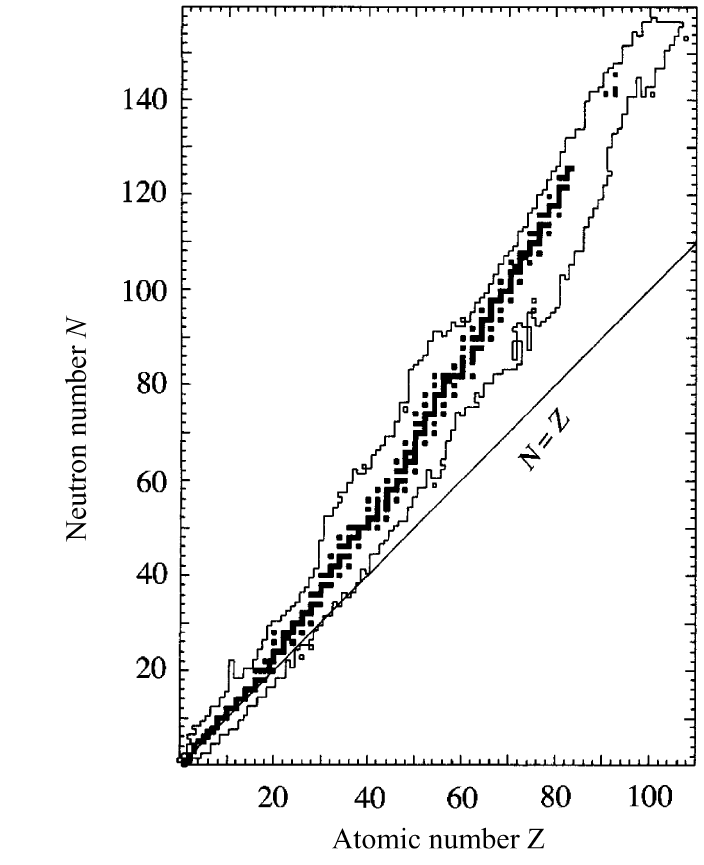
\includegraphics[width=0.6\linewidth]{figures/nuclidmap}
    \caption{Nuclid map of stable nuclei \cite{Hooshyar}: The squares are the long-lived nuclei
    occuring in nature; other known nuclei lie within the jagged lines and are unstable.}
    \label{fig:nuclidmap}
\end{figure}
\label{ssub:Semi-Empirical Mass Formula: The Liquid Drop Model}
Going along with  \cite{Hooshyar}, we approach a theoretical model containing constants which
have to be fitted with experiments. For this reason, the model is called semi-empirical. 
It was first established by Weizsäcker and yields a 
good approximation for the atomic masses. The assumptions underlying are:
\begin{enumerate}
    \item All nuclei have approximately the same interio mass density.
        \label{it1}
    \item Their total binding energies are approximately proportional to their masses.
        \label{it2}
\end{enumerate}
Both turnout to be valid in the regime we are looking at.
The assumptions show why the model is called \emph{liquid drop model}: 
(\ref{it1}) is the analogue of regarding the nuclei as incompressible fluids, 
(\ref{it2}) is related to the proportionality of latent heats of vaporization to the masses of a drop. 
We construct the energy in units of masses with different contributions:
\begin{equation}
    M_{tot} = \sum_{i=0}^{5} f_i 
\end{equation}
\begin{itemize}
    \item \textbf{Mass term:} 
First we take into account the atomic masses 
consisting of the mass of the nucleons and electrons:
\begin{equation}
    f_0 = Z(M_p + m_e) + (A-Z)M_n
\end{equation}
    \item \textbf{Volume term:} This term will estimate the effect of strong 
        nuclear forces proportional to the volume:
        \begin{equation}
            f_1 = -a_1 A\, ,
        \end{equation}
        where $a_1$ has to be found depending on the volume. 
    \item \textbf{Surface term:} 
        This term corrects the volume energy by a surface term
        \begin{equation}
            f_2 = a_2 A^{\frac{2}{3}} 
        \end{equation}
        taking into account that in binding energy is lowered as nuclei at the surface 
        have fewer interaction partners. The analogue is the surface tension energy 
        in the classical liquid drop model.
    \item \textbf{Coulomb term:} The protons of each nucleus repell each other due to the 
        electrostatic Coulomb force.If we assume a uniform charge distribution of 
        radius proportional to $A^{\frac{1}{3}}$, then
        \begin{equation}
            f_3 = a_3 \frac{Z(Z-1)}{A^{\frac{1}{3}}} \approx a_3 \frac{Z^2}{A^{\frac{1}{3}}} 
            \qquad (\text{for} \quad Z \gg 1)
        \end{equation}
    \item \textbf{Assymetric term:} Due to the Pauli principle the nuclei tend to broaden their distribution
        on energies, with leads to a positive energy correction for more assymetric numbers $A$ and $Z$:
        \begin{equation}
            f_4 = a_4 \frac{(Z- \frac{A}{2})^2}{A}
        \end{equation}
    \item \textbf{Pairing term:} This correction accounts for the tendency of proton pairs and neutron pairs
        to occur, where an even number of particles is more stable than an odd number:
      \begin{equation}
          f_5   =
          \begin{cases}
              -f(A) & \text{if $Z$ even and $A-Z=N$ even}\\
              0     & \text{if $Z$ even but $A-Z=N$ odd or $Z$ odd but $A-Z=N$ even}\\
              f(A)  & \text{if $Z$ odd and $A-Z=N$ odd}
          \end{cases}
          \label{eq:pair}
      \end{equation}
      The function $f(A)$ should be estimated by fitting the data, 
      often $f(A) = a_5 A^{-\frac{1}{2}}$ is used.
\end{itemize}

\subsubsection{Unstable States}
\label{ssub:Unstable States}
If we want investigate the form of the energy distribution of a decay, we have to 
introduce the \emph{natural decay width}, given by
\begin{equation}
    \Gamma_f = \frac{\hbar}{\tau_f} 
\end{equation}
which can be defined for each channel $f$, such that in total we get
\begin{equation}
    \Gamma = \sum_{f} \Gamma_f \, .
\end{equation}
We can define the \emph{branching ratio} for channel $f$ by
\begin{equation}
    B_f = \frac{\Gamma_f}{\Gamma} \, .
\end{equation}
The energy distribution of the unstable state to a final state $f$ resolves into a 
\emph{Breit-Wigner-distribution}: 
\begin{equation}
    N_f(M_f) = \frac{\Gamma_f}{(M_f-M_i)^2 c^4 + \Gamma_f^2/4}
\end{equation}
with the mass of the decaying state $M_i$ and the invariant mass of decay products $M_f$.
\begin{figure}[htpb]
    \centering
    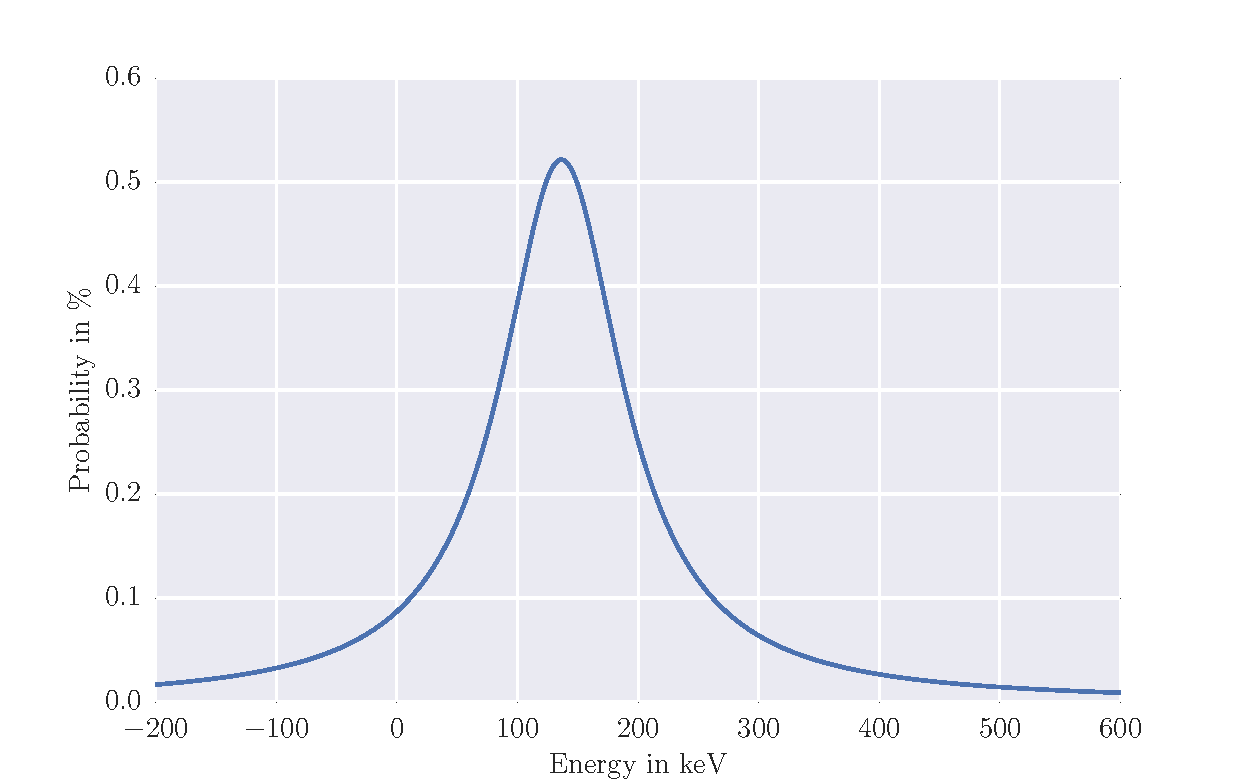
\includegraphics[width=0.9\linewidth]{analysis/figures/breit_wigner}
    \caption{Breit-Wigner distribution. Here again with
        $^{57}Cs\rightarrow ^{57}Fe$ with $t_{1/2}=270$. Hence we have $M_i = 136.5$keV and
    $\Gamma_f = \hbar / \textrm{log}(2)t_{1/2} = 122$keV, which resamples in the width of the curve.}
    \label{fig:name}
\end{figure}
\clearpage

\subsection{Overview of technical instruments}
We will give a short overview over the technical instruments used. The exact role 
of the devices will be explained in section thereafter.
\label{sub:overview_of_technical_instruments}
\paragraph{Scintillator}
In order to detect the $\gamma$ - rays from a radioactive sample, we use a widely used detector called/
\emph{scintillator}. The name refers to a quality of the material used: The \emph{scintillation}, or production 
of flashes of light induced by the passing $\gamma$ photons. 
The energy of incoming particles
is adsorbed and released at a lower frequency (ideally in the visible or UV-spectrum). 
We can measure the energy as well as the time of detection. 
In our case we use the organic crystal \textbf{NaI(Tl)} as scintillator, which
is preferable because of its high yield~\cite{ver} in comparison to others. However, the decay time is longer
than for organic scintillatiors, which is not a problem in our case since the low activity of our probe will
not result in (a measurable quantity of) jammed photons.
In the detector, this material is coupled to a photomultiplier in order
to gain an measurable signal. 

\paragraph{The Photomultiplier}
will be used to amplify the signal from the scintillator. It is built upon
two fundamental physical phenomena: The \textit{photoeffect} and the \textit{secondary emission}. While the former
is well known due to its scientific father\footnote{Despite the effect that Heinrich Hertz discovered the 
Photoeffect 1887, Albert Einstein published an explanation 1905 with which he shows the quantum character
of light. 1921 he was rewarded the Nobel Price in physics.}, the latter is less popular: Particles (with
sufficient energy) induce the emission of secondary particles while going through a specific material. In
our case the primary particles will be the photons emitted by the scintillator, while the secondary induced
in the photomultiplier are electrons. These electrons are accelerated towards an electrode (which is called
\textit{dynode} in this special case) in order to induce the emission of further electrons. 
The process is repeated over and over such that even single photons can be detected clearly
(see figure~\ref{fig:photomultiplier} for a schematic diagram).
Depending on the experimental setup it is possible to amplify a signal by eight orders of magnitude. 
\begin{figure}[htpb]
    \centering
    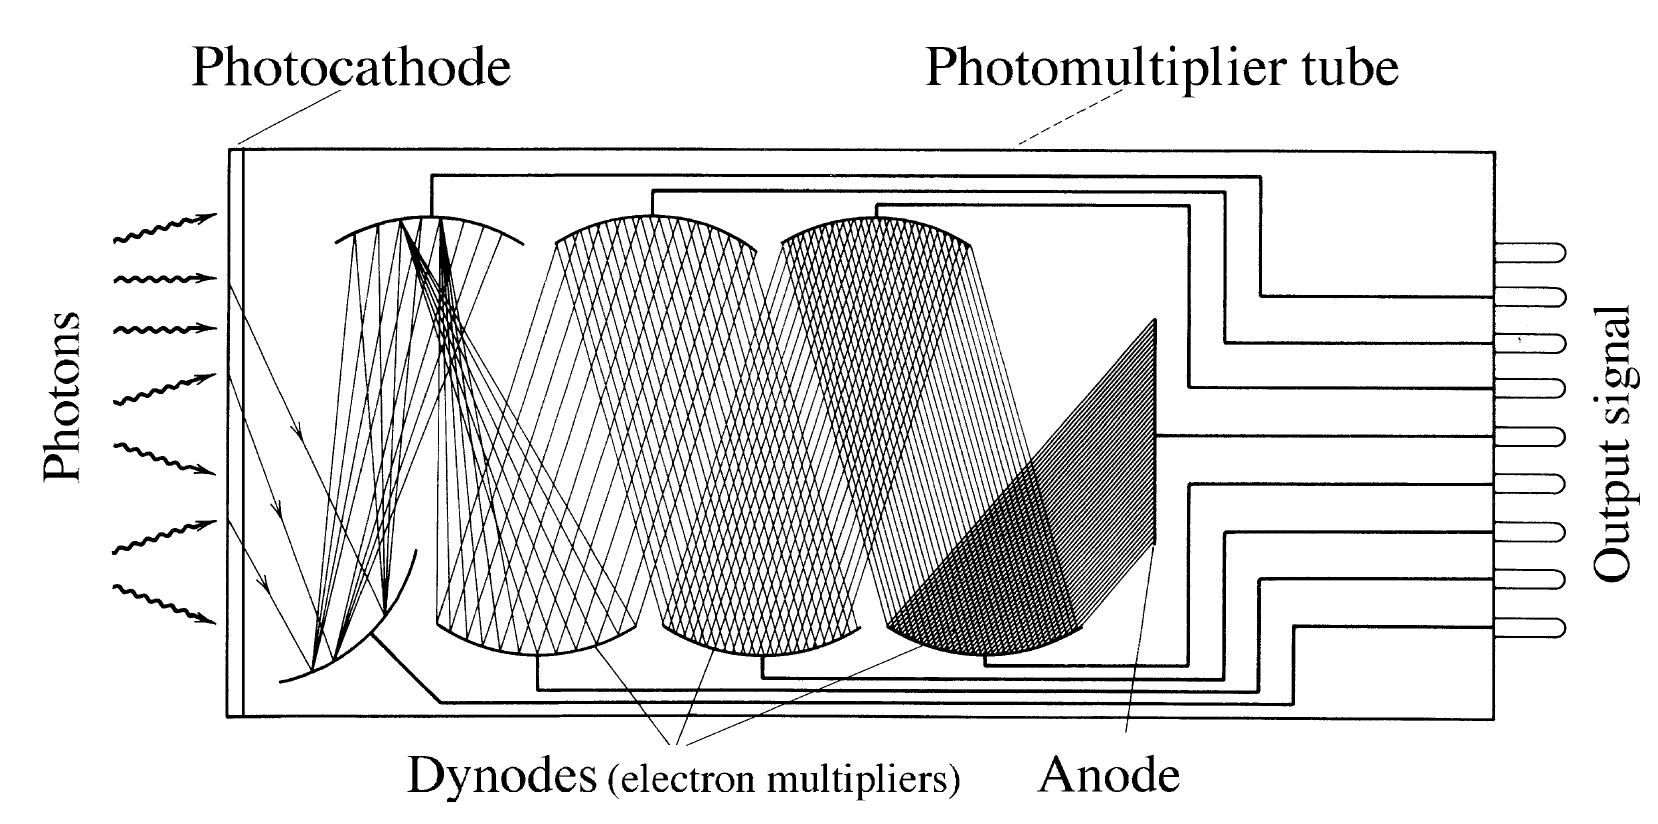
\includegraphics[width=0.8\linewidth]{figures/photomultiplier}
    \caption{
        Schematic diagram of a photomultiplier tube. The incoming photons are translated into electrons, 
        which are accelerated towards the
        next dynode such that more and more electrons are induced to amplify the signal.
        Taken from~\cite{bettini2008introduction}. 
        }
    \label{fig:photomultiplier}
\end{figure}
\paragraph{The Single Channel Analyzer (SCA)} is the next instrument to process the signal detected. In general
it refers to a electronic component creating a outputsignal only when the amplitude (of the input) happens to be
between predefined constraints. Hence the SCA is a binary unit. We will use it amongst others for
applying an energy window to the spectrum in order to indentify certain peaks with events. 
\paragraph{The Time-to-amplitude Converter (TAC)} is the missing link between energies detected by the scintillator
and times. It is possible to convert the amount of time between a start and a stop signal into an amplitude,
which can be further analyzed statistically. The component was developed by a famous italian physicist%
\footnote{1942 Bruno Rossi invented the TAC in order to ascertain the half life period of mesons. The first
    experiment of this kind was done in similar fashion as ours: The time difference between the
    arrival of a meson in an absorber and its decay through an electron emission was measured with an
    electronic circuit producing an amplitude proportional to the time interval. Quoting Rossi:
    \textit{``How is it possible that results bearing on fundamental problems of
        elementary particle physics could be achieved by experiments of an almost childish simplicity,
        costing only a few thousand dollars and requiring only the help of one or two graduate students? ``}}
and is used especially because of the linear relationship betwen amplitude and real time, a quality we will also
show in a measurement.
\paragraph{Multi Channel Analyzer (MCA)} are used intensively for sorting a stream of voltage pulses
into a histogram, integrating over a specific amount of time. The stored number of events versus pulse-height
can be analyzed afterwards.
